\section{Fase di Progettazione}
    \subsection{Struttura del Sito}
    In questa sezione presentiamo una prima bozza grafica delle varie pagine del sito. Ciò ci è servito per avere un'idea generale sull'aspetto che dovrà avere il sito e per avere una base da cui partire per lo sviluppo del layout.

    \begin{center}
        \begin{minipage}{0.4\linewidth}
            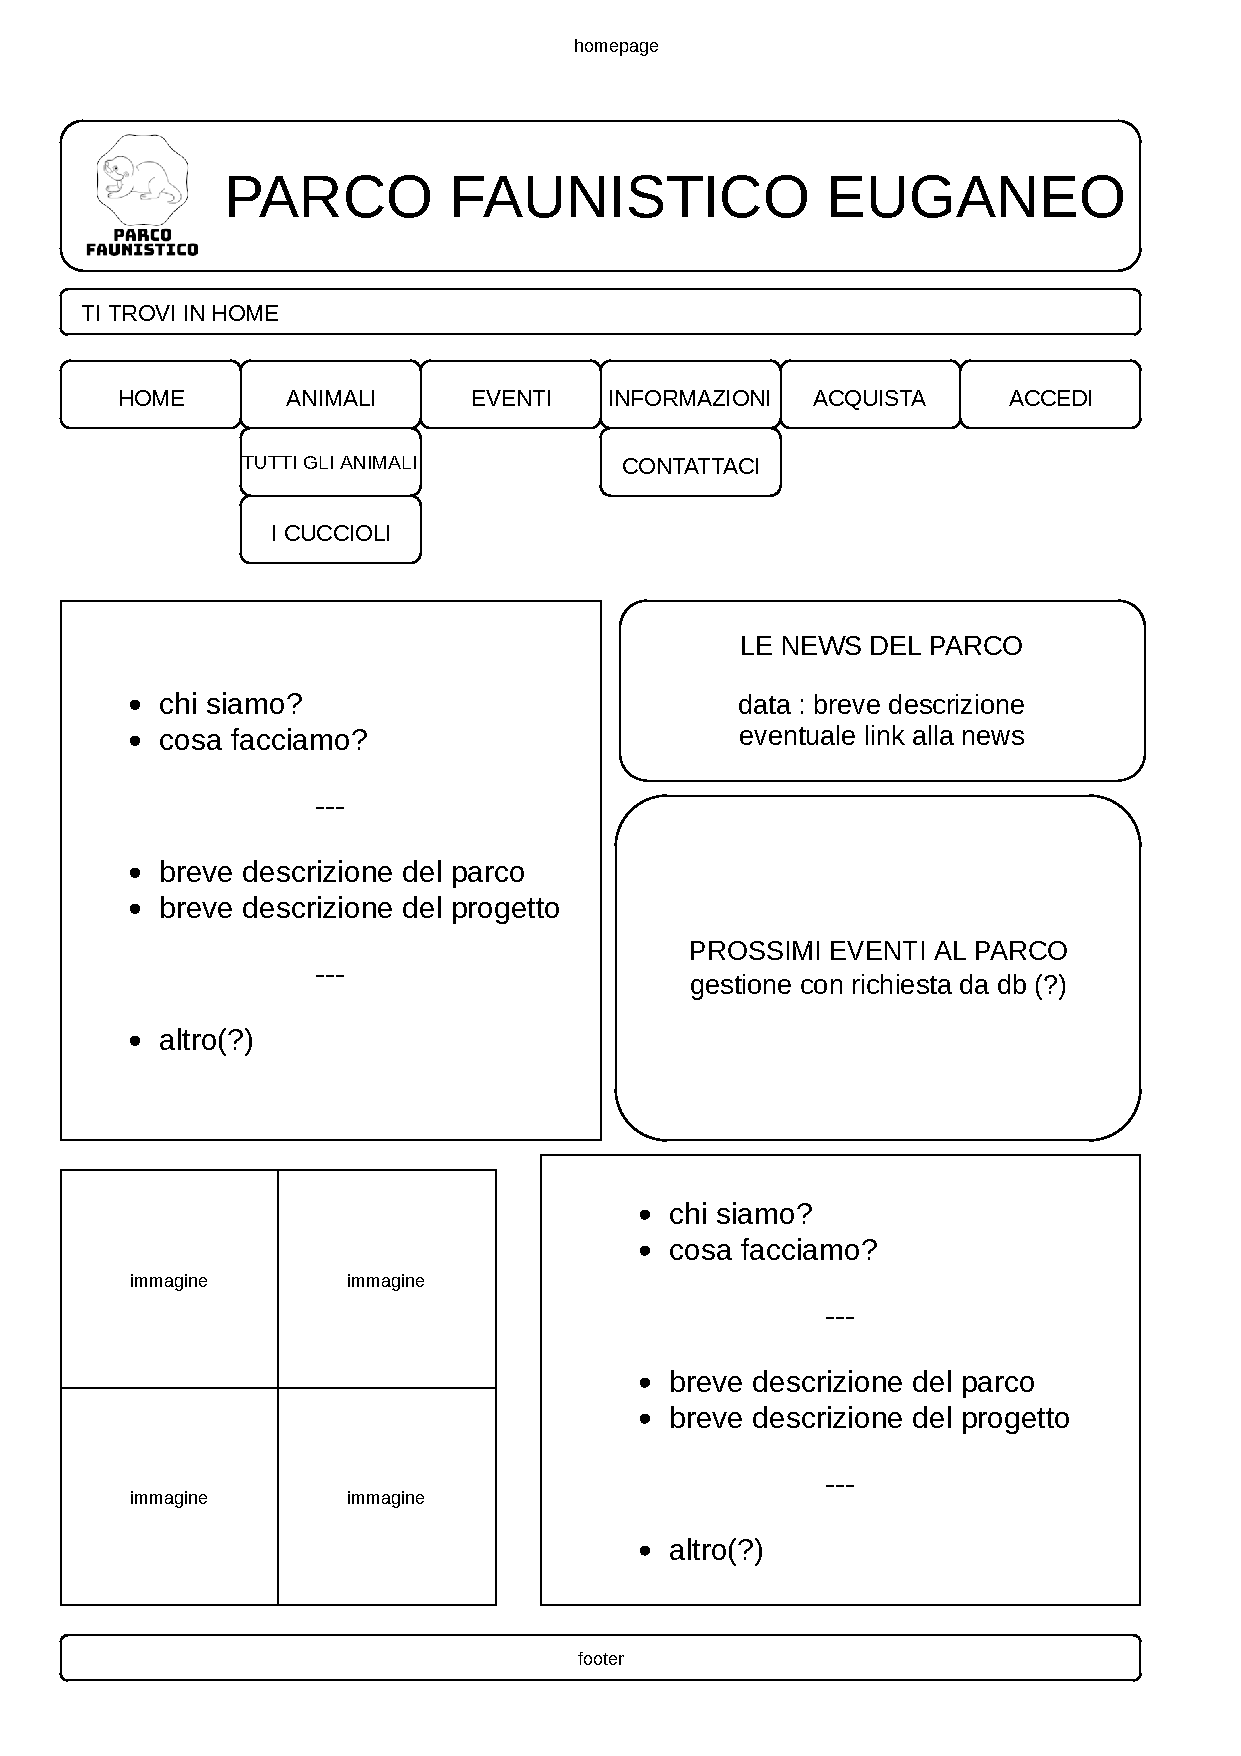
\includegraphics[width=\linewidth]{./../docs/Analisi/bozze/homepage.pdf}
            \captionof{figure}{Homepage}
        \end{minipage}%
        \hfill
        \begin{minipage}{0.4\linewidth}
            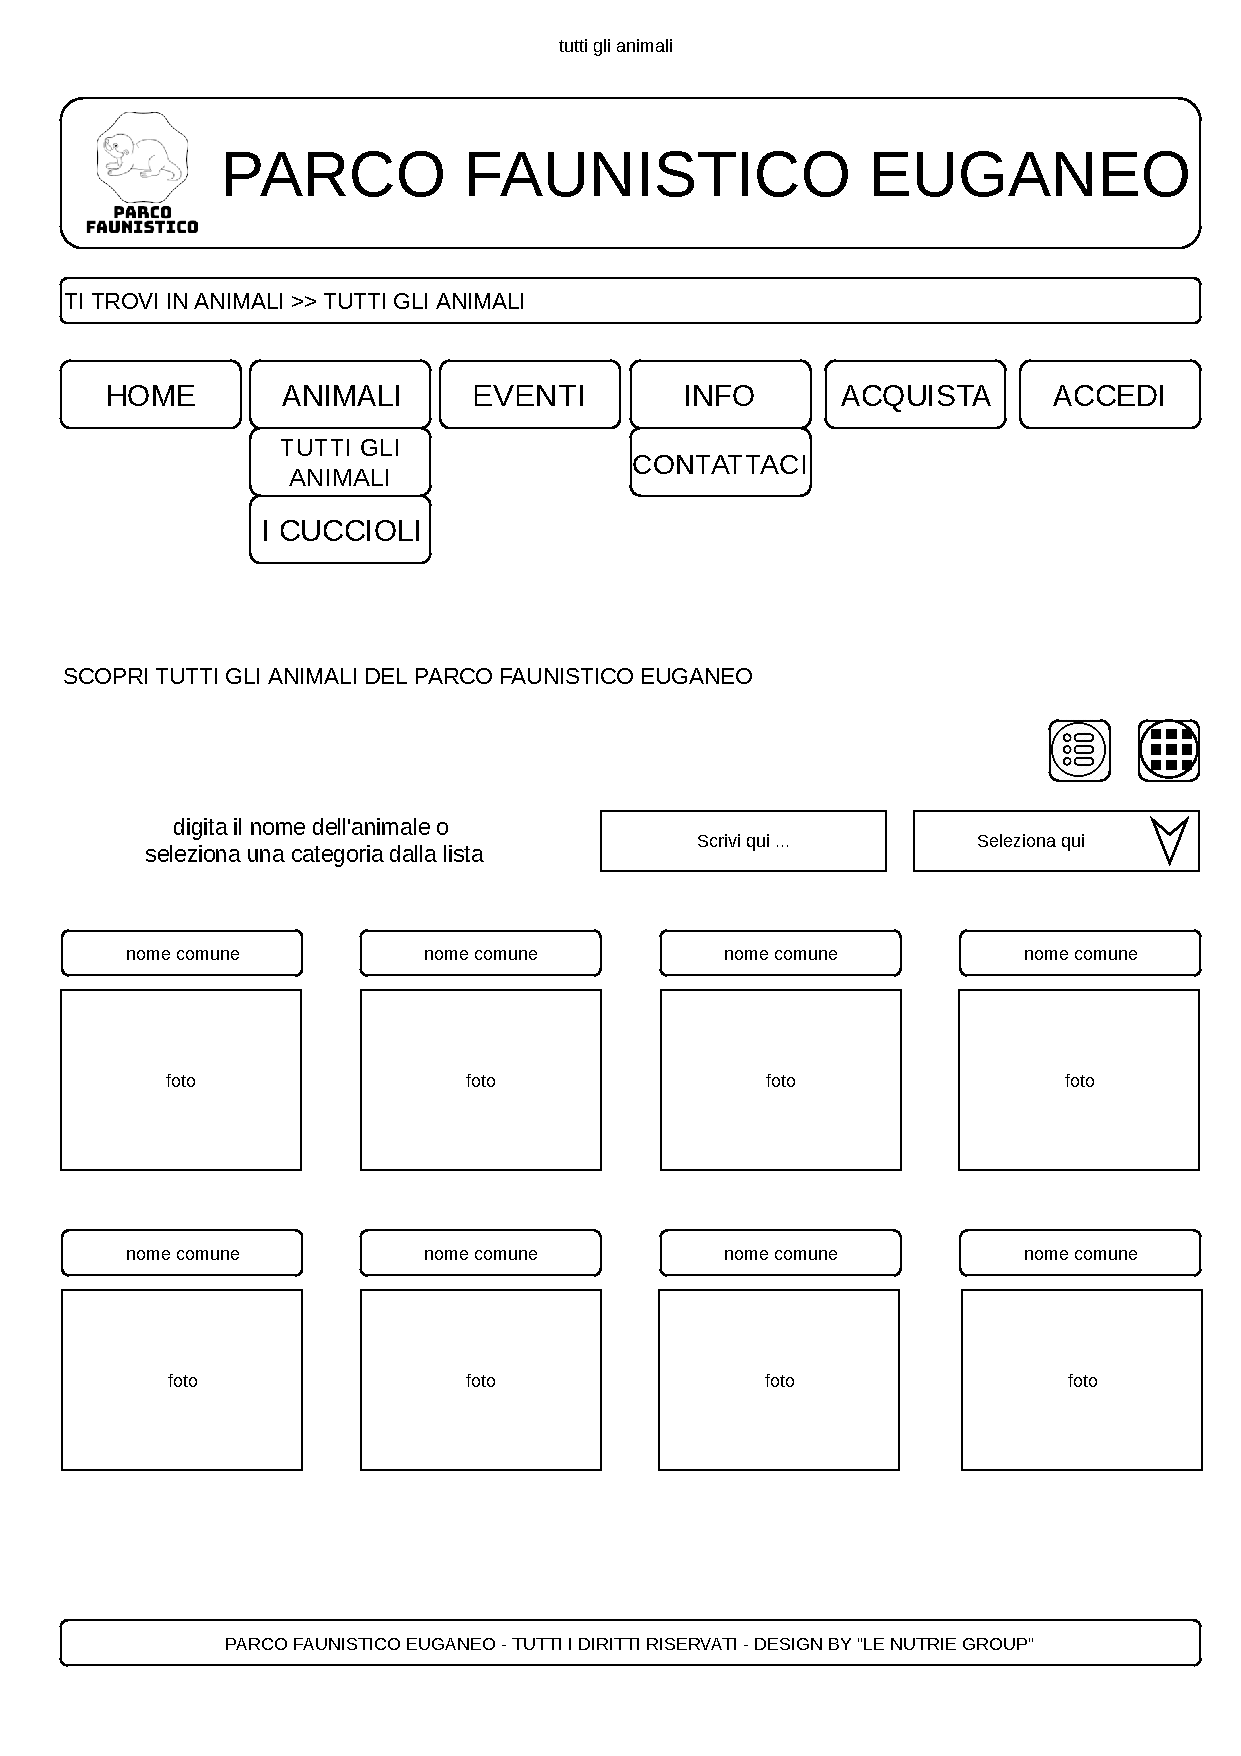
\includegraphics[width=\linewidth]{./../docs/Analisi/bozze/animali-grid.pdf}
            \captionof{figure}{Animali vista griglia}
        \end{minipage}
        \hfill
        \begin{minipage}{0.4\linewidth}
            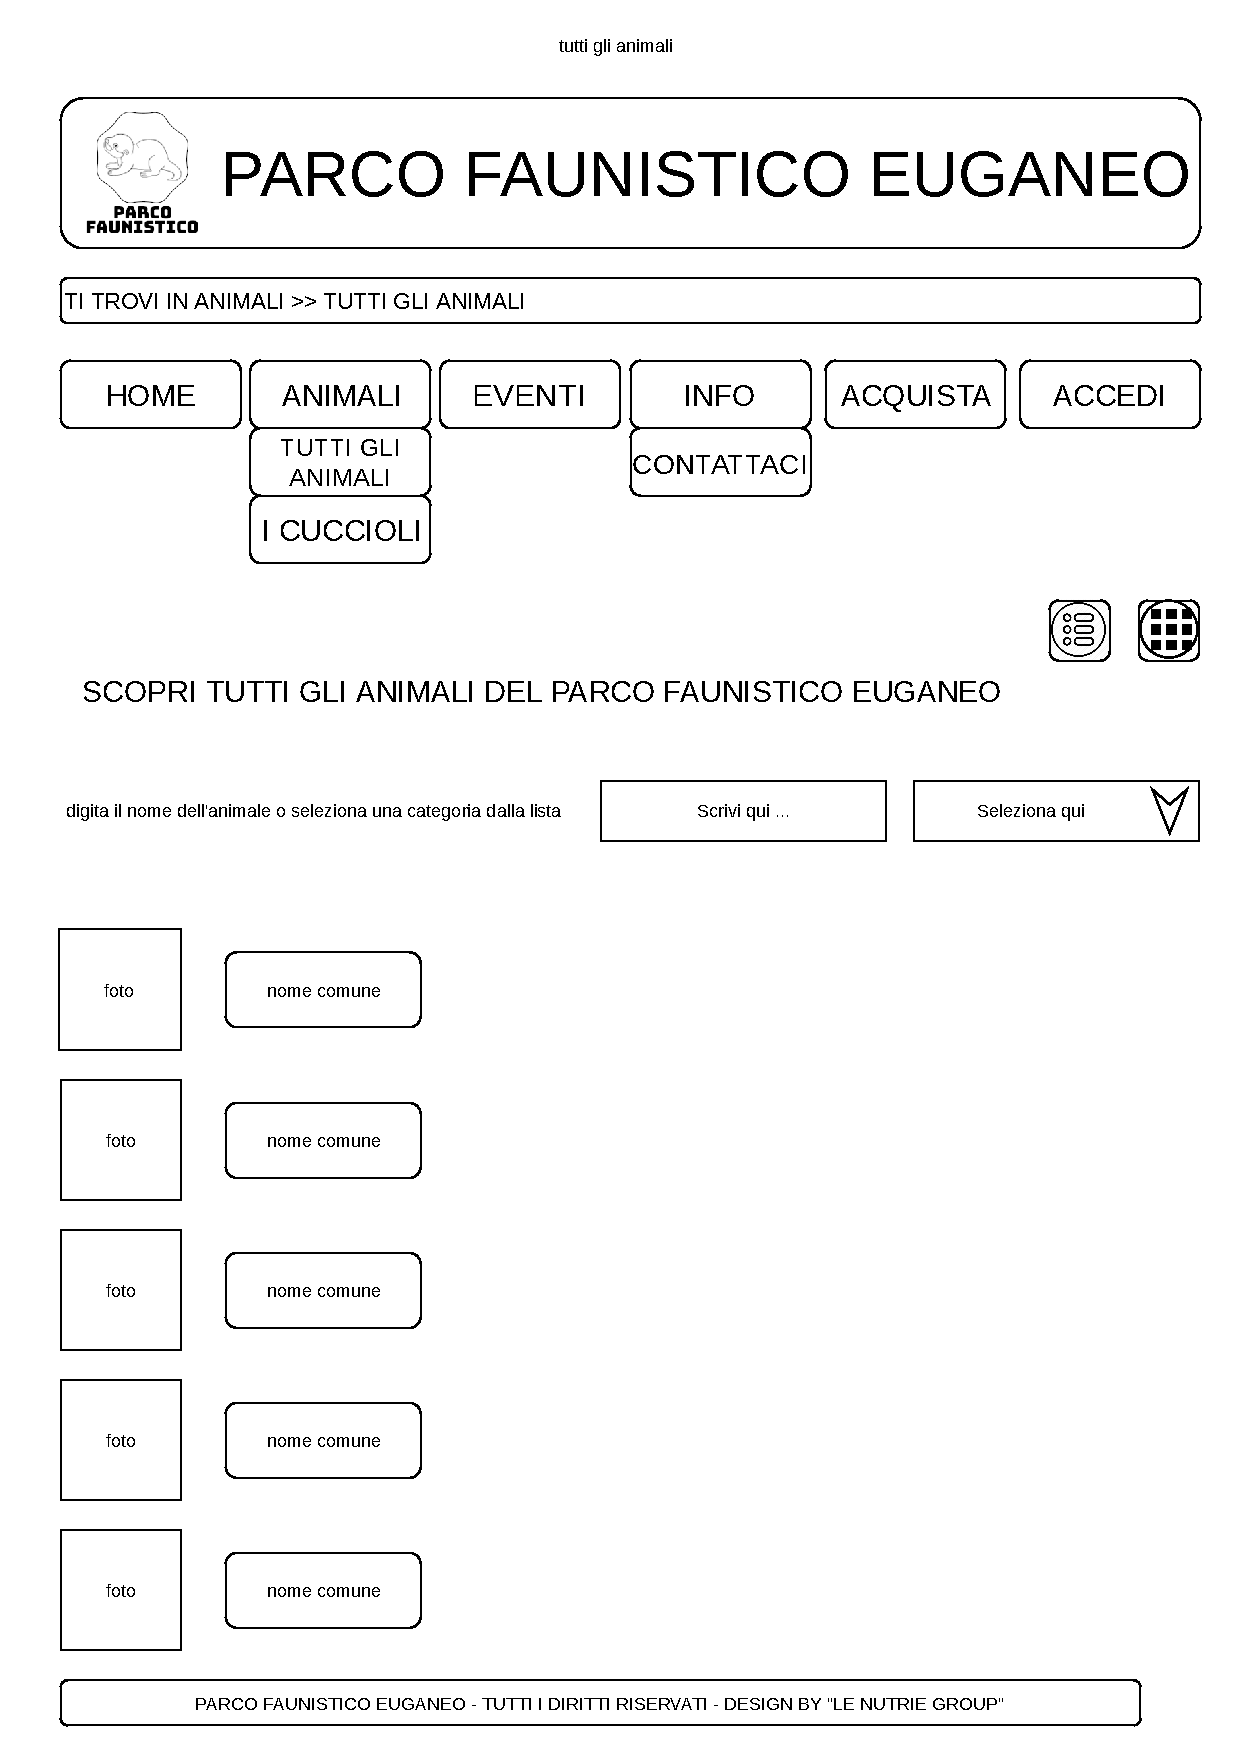
\includegraphics[width=\linewidth]{./../docs/Analisi/bozze/animali-list.pdf}
            \captionof{figure}{Animali vista lista}
        \end{minipage}%
        \hfill
        \begin{minipage}{0.4\linewidth}
            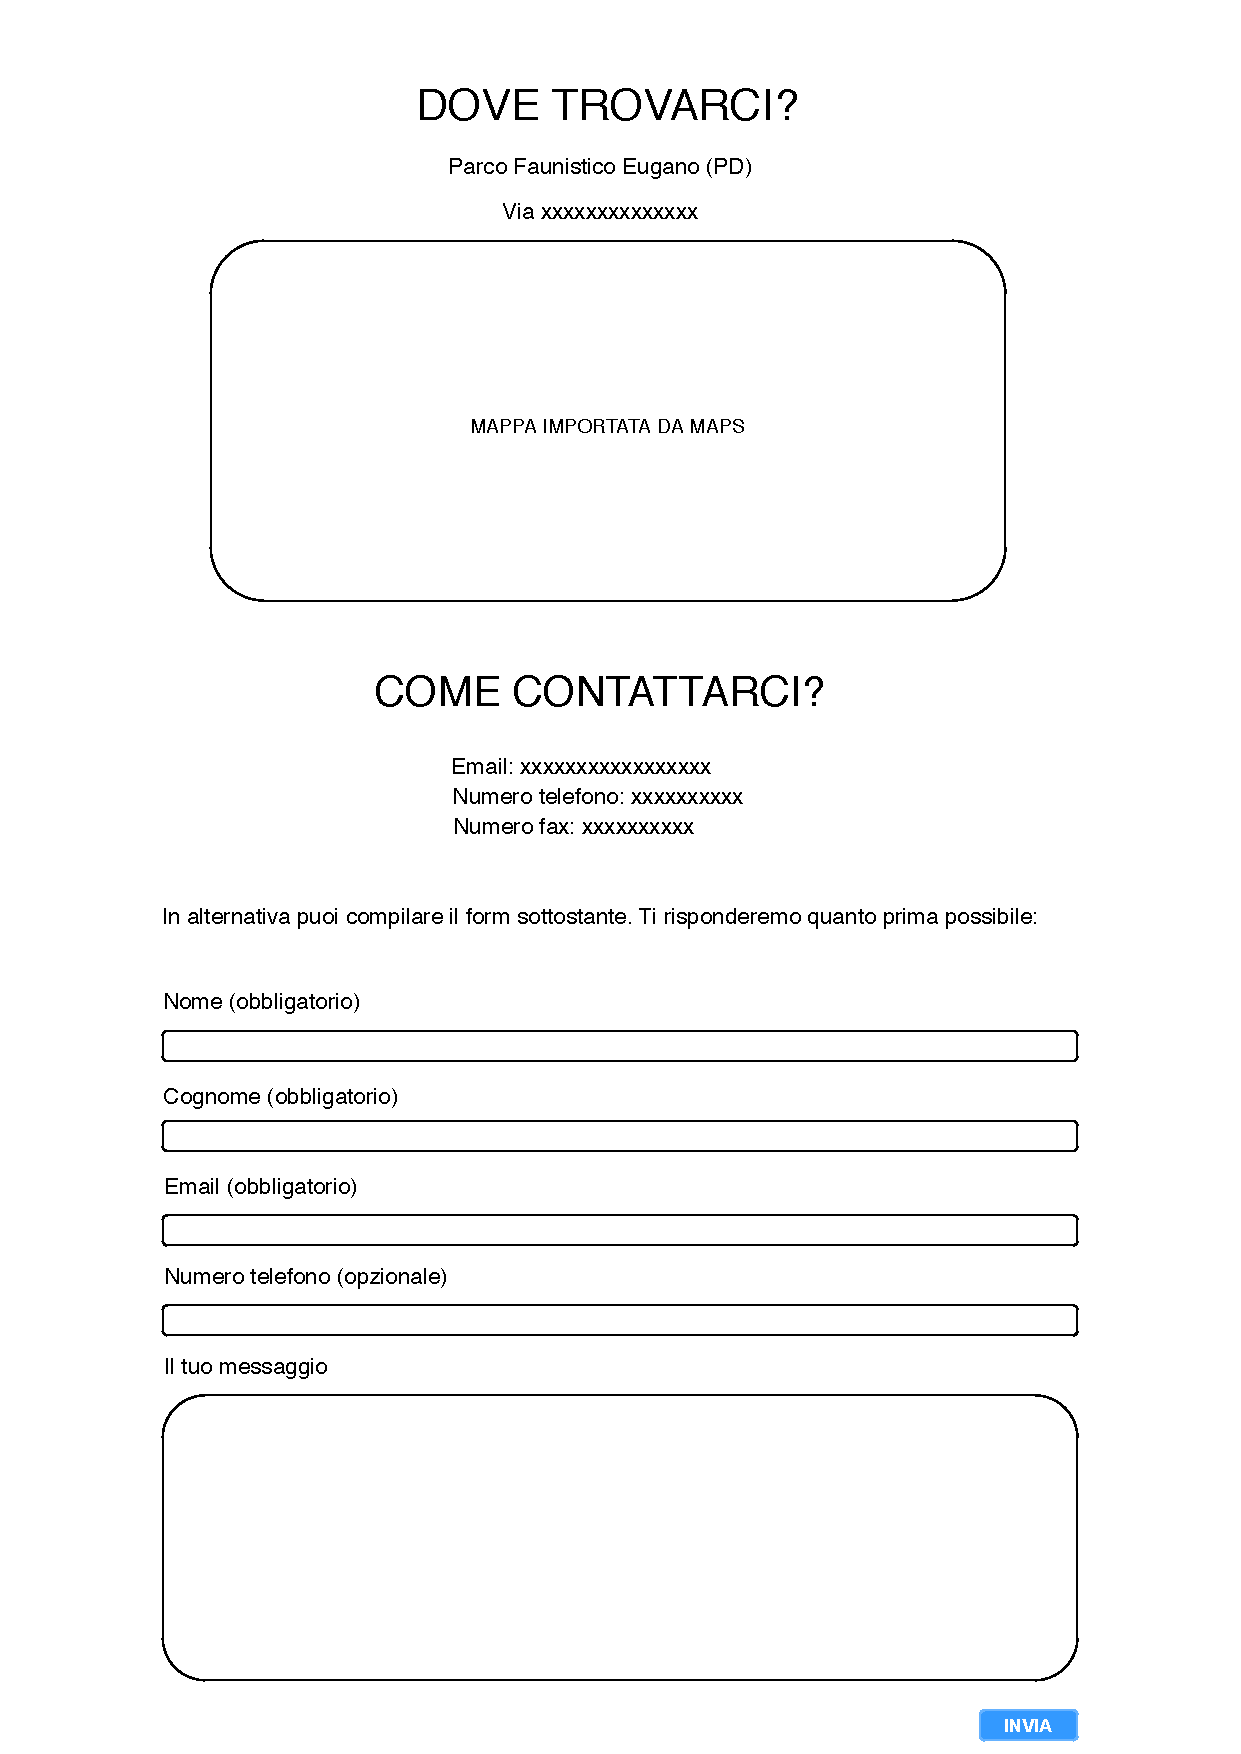
\includegraphics[width=\linewidth]{./../docs/Analisi/bozze/Info.pdf}
            \captionof{figure}{Informazioni}
        \end{minipage}%
        \hfill
        \begin{minipage}{0.4\linewidth}
            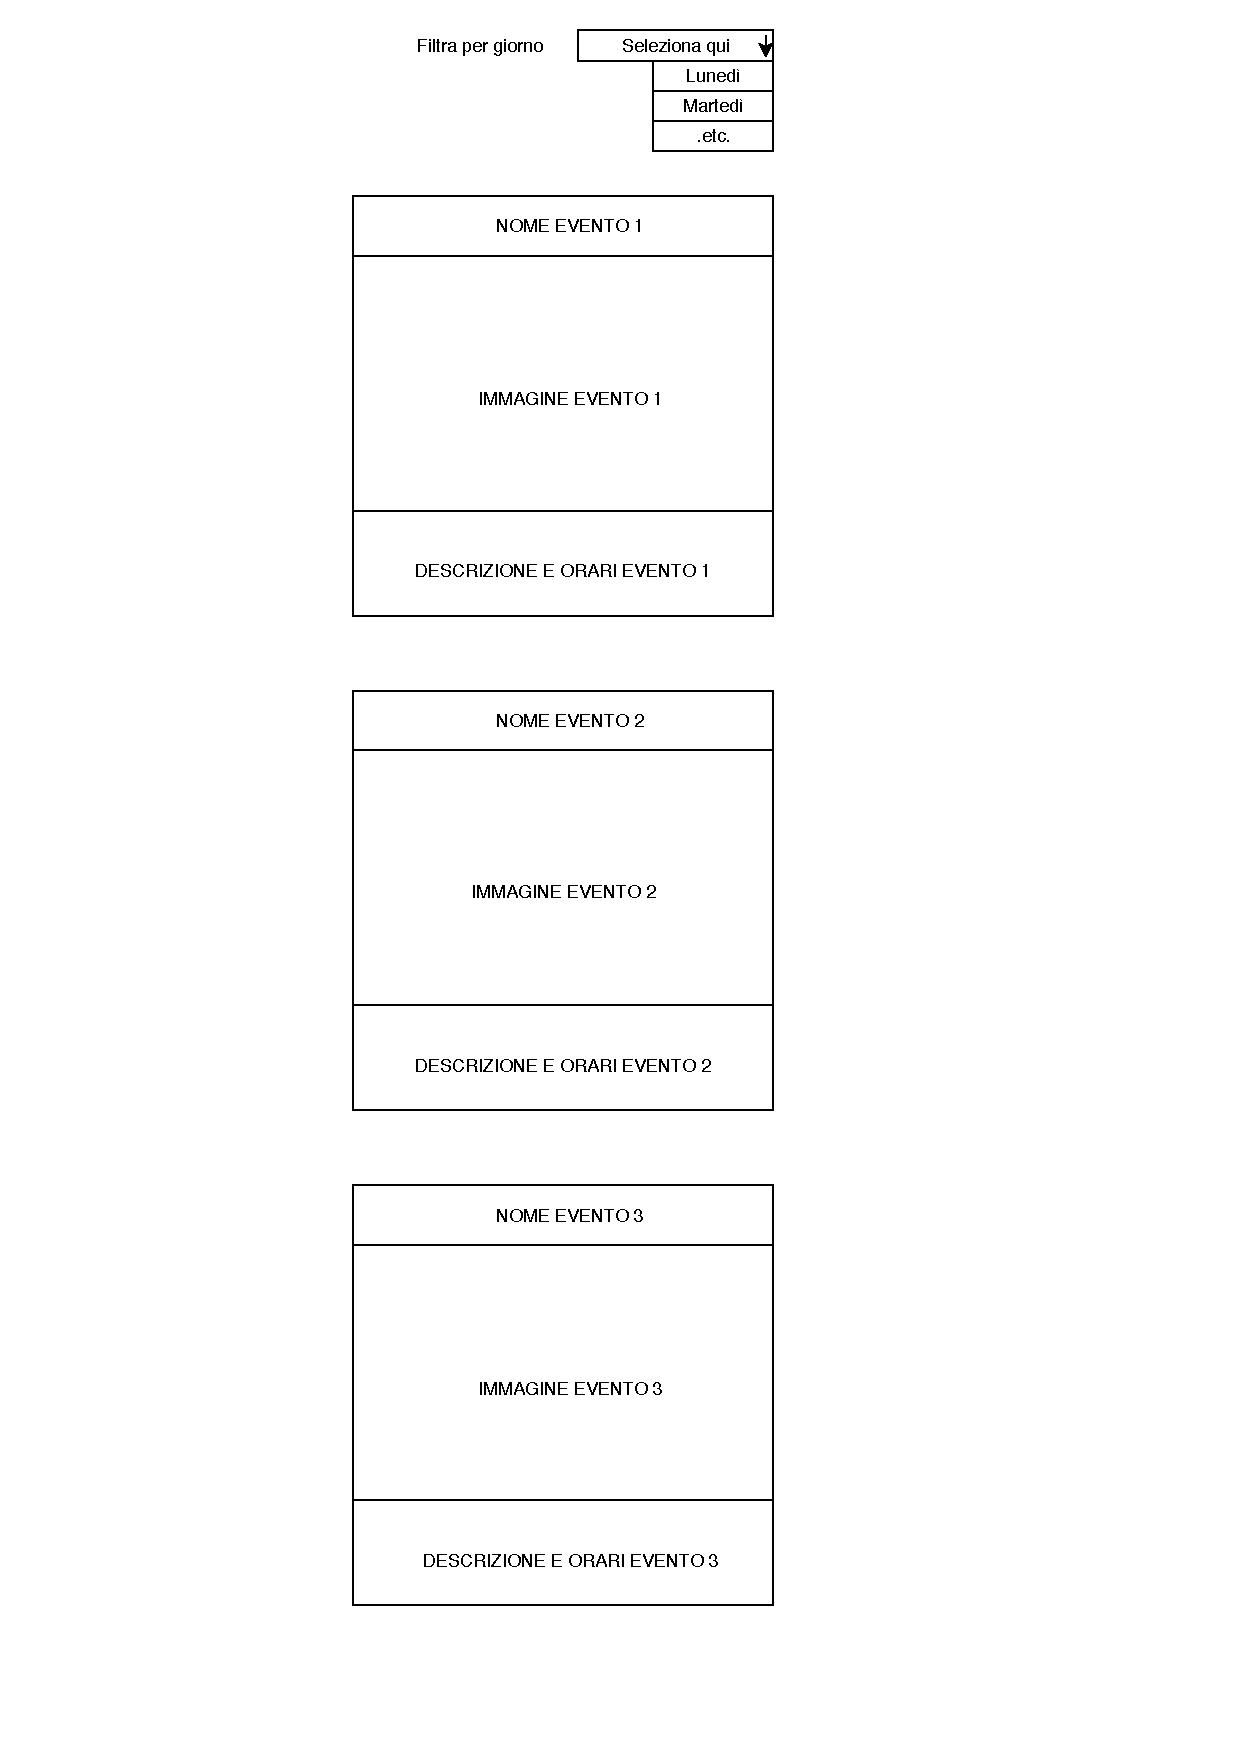
\includegraphics[width=\linewidth]{./../docs/Analisi/bozze/Eventi.pdf}
            \captionof{figure}{Eventi}
        \end{minipage}%
        \hfill
        \begin{minipage}{0.4\linewidth}
            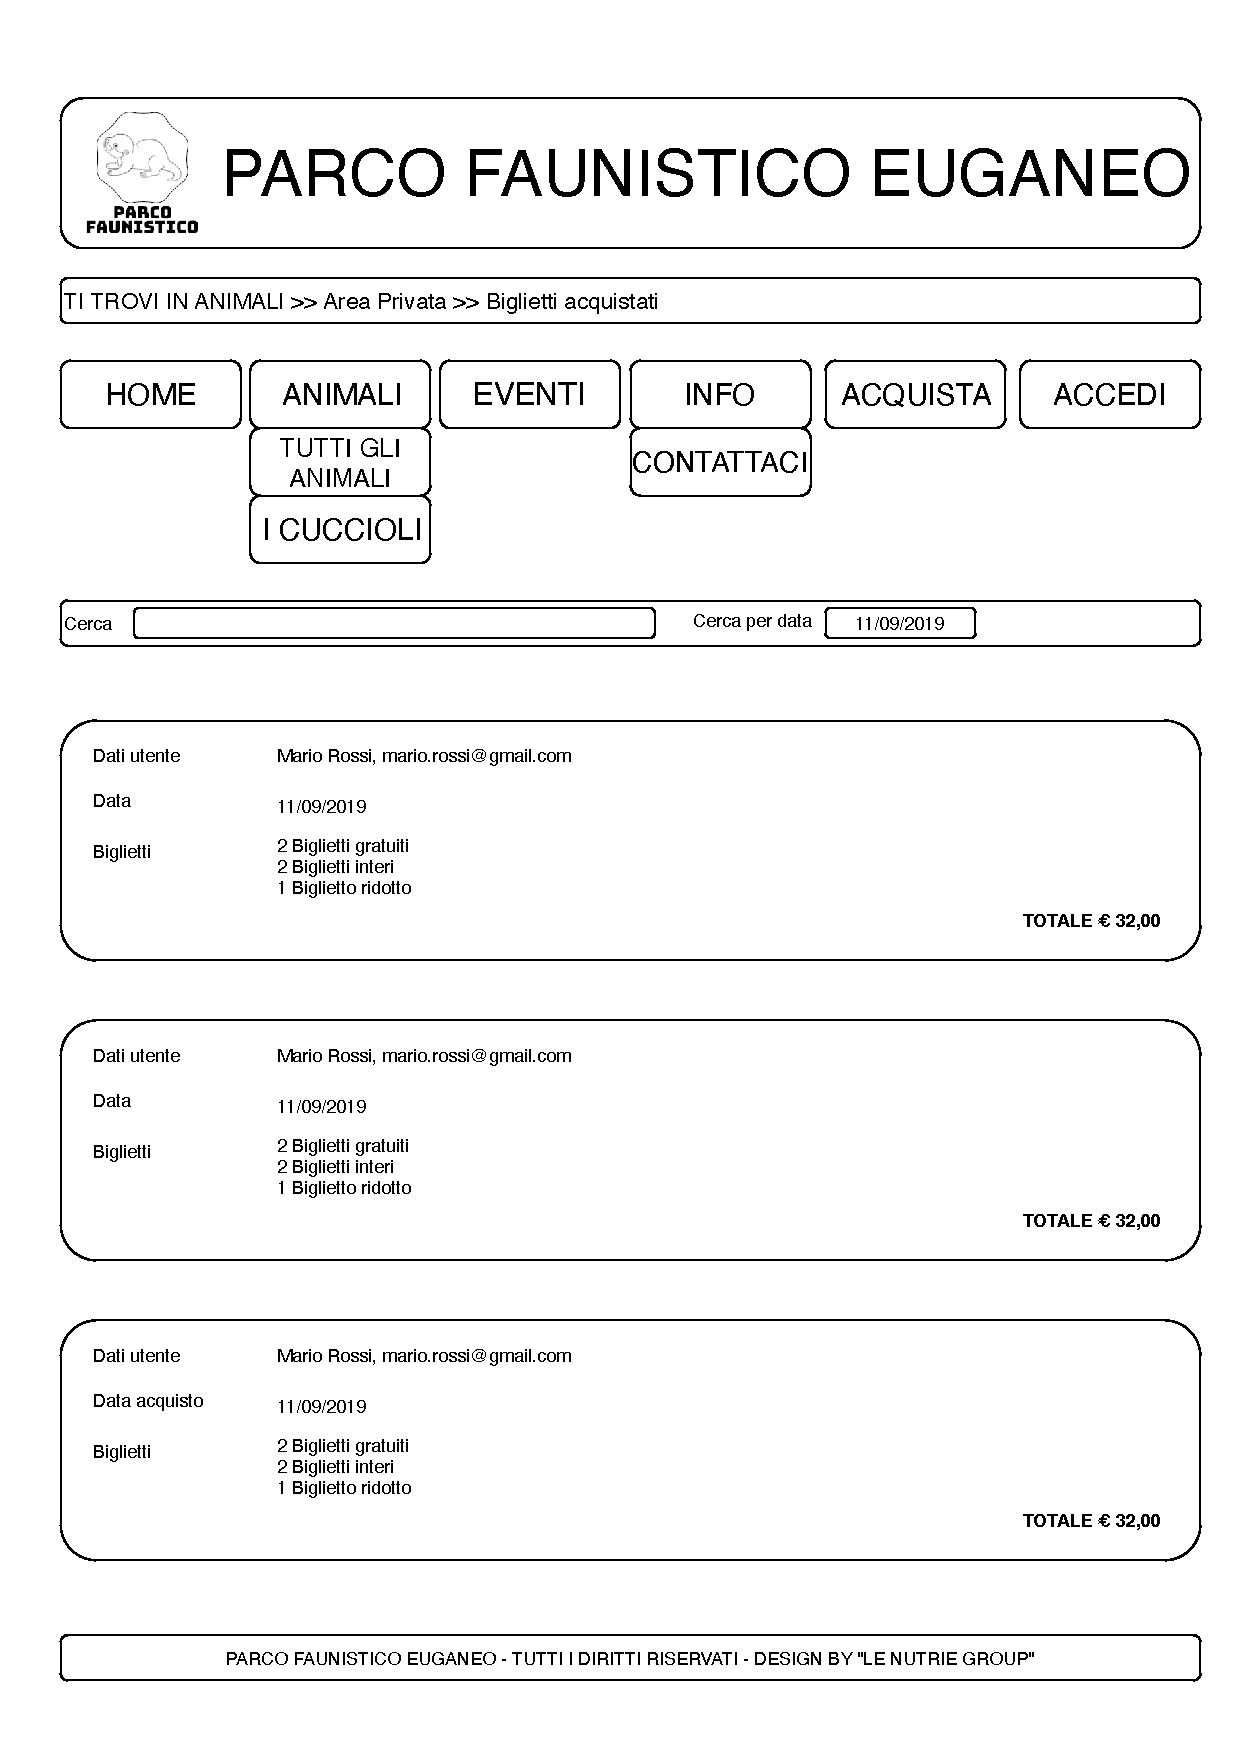
\includegraphics[width=\linewidth]{./../docs/Analisi/bozze/riepilogoAcquisti.pdf}
            \captionof{figure}{Acquista}
        \end{minipage}
        \hfill
        \begin{minipage}{0.4\linewidth}
            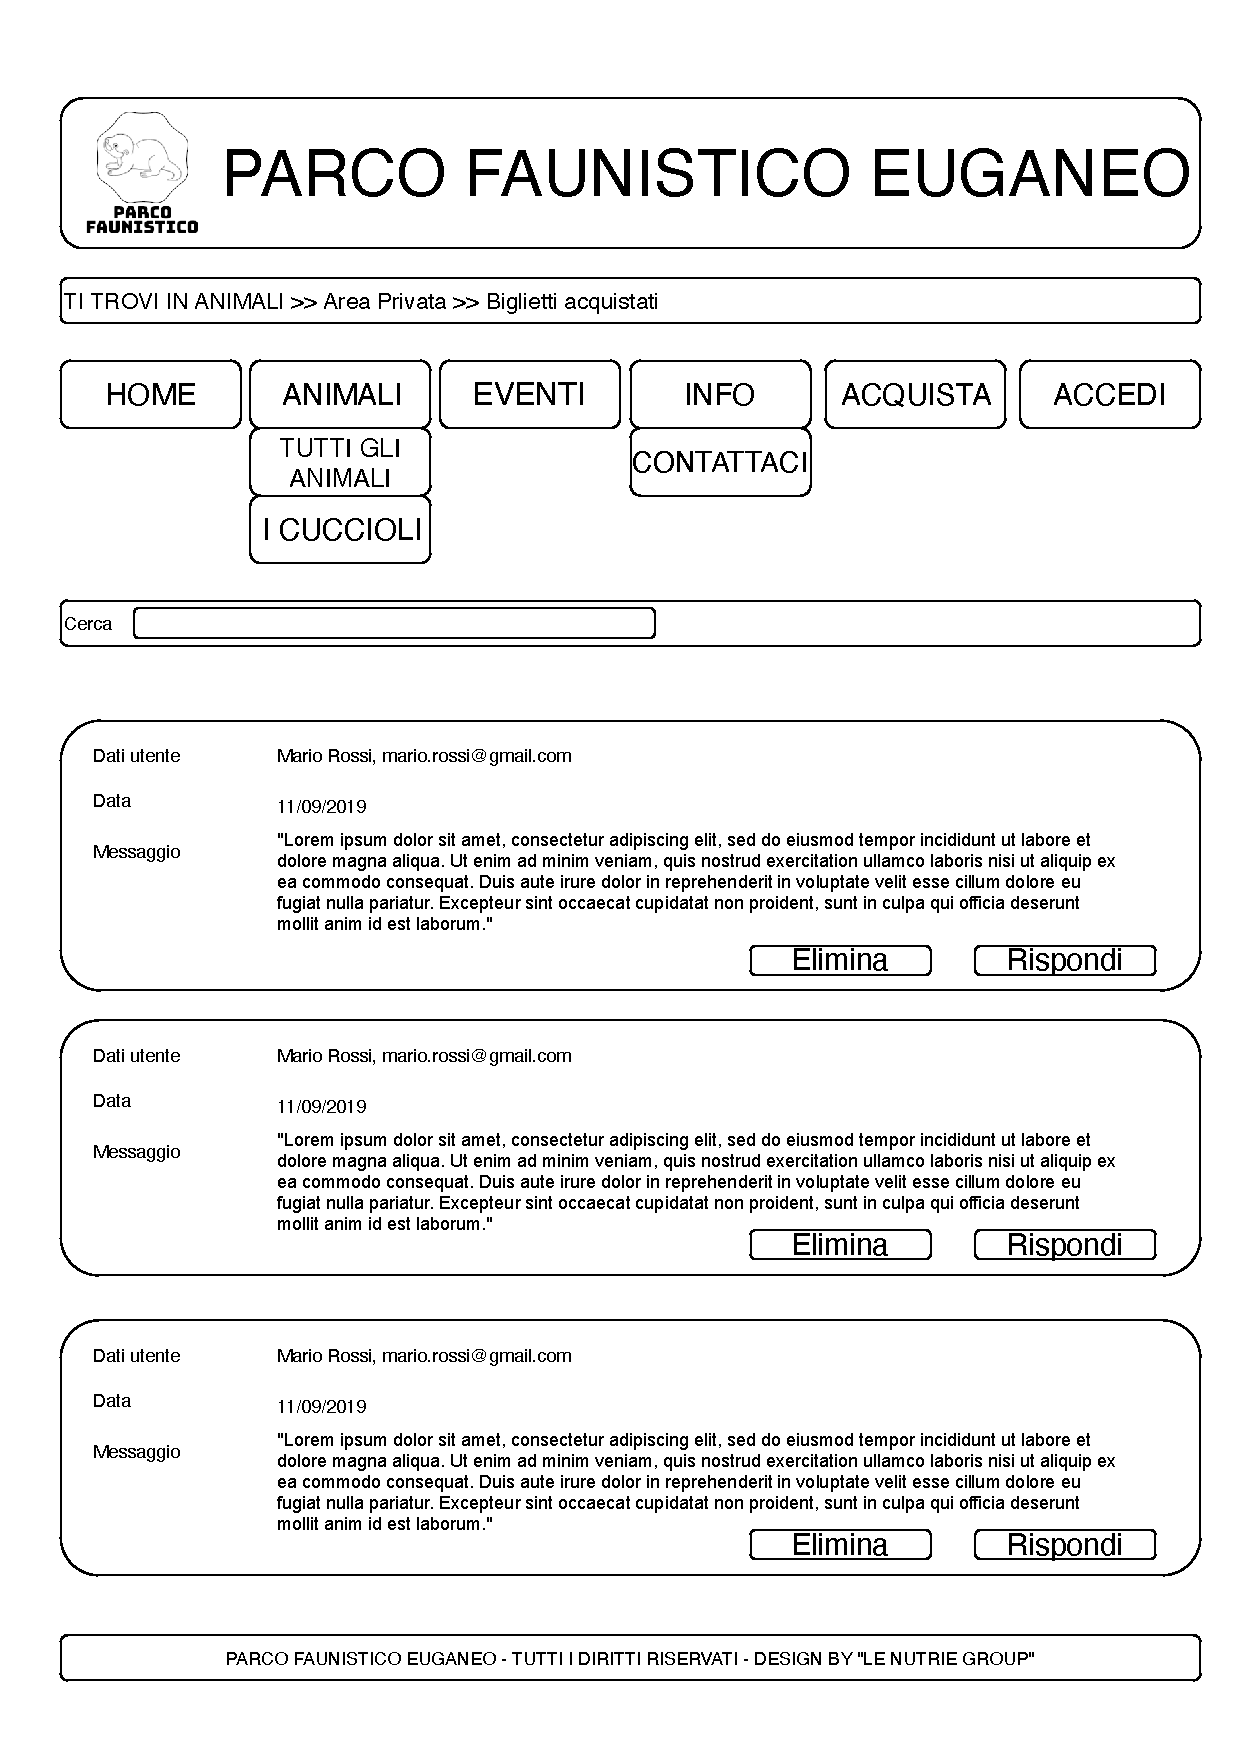
\includegraphics[width=\linewidth]{./../docs/Analisi/bozze/Messaggi.pdf}
            \captionof{figure}{Area Privata - Messaggi}
        \end{minipage}%
        \hfill
        \begin{minipage}{0.4\linewidth}
            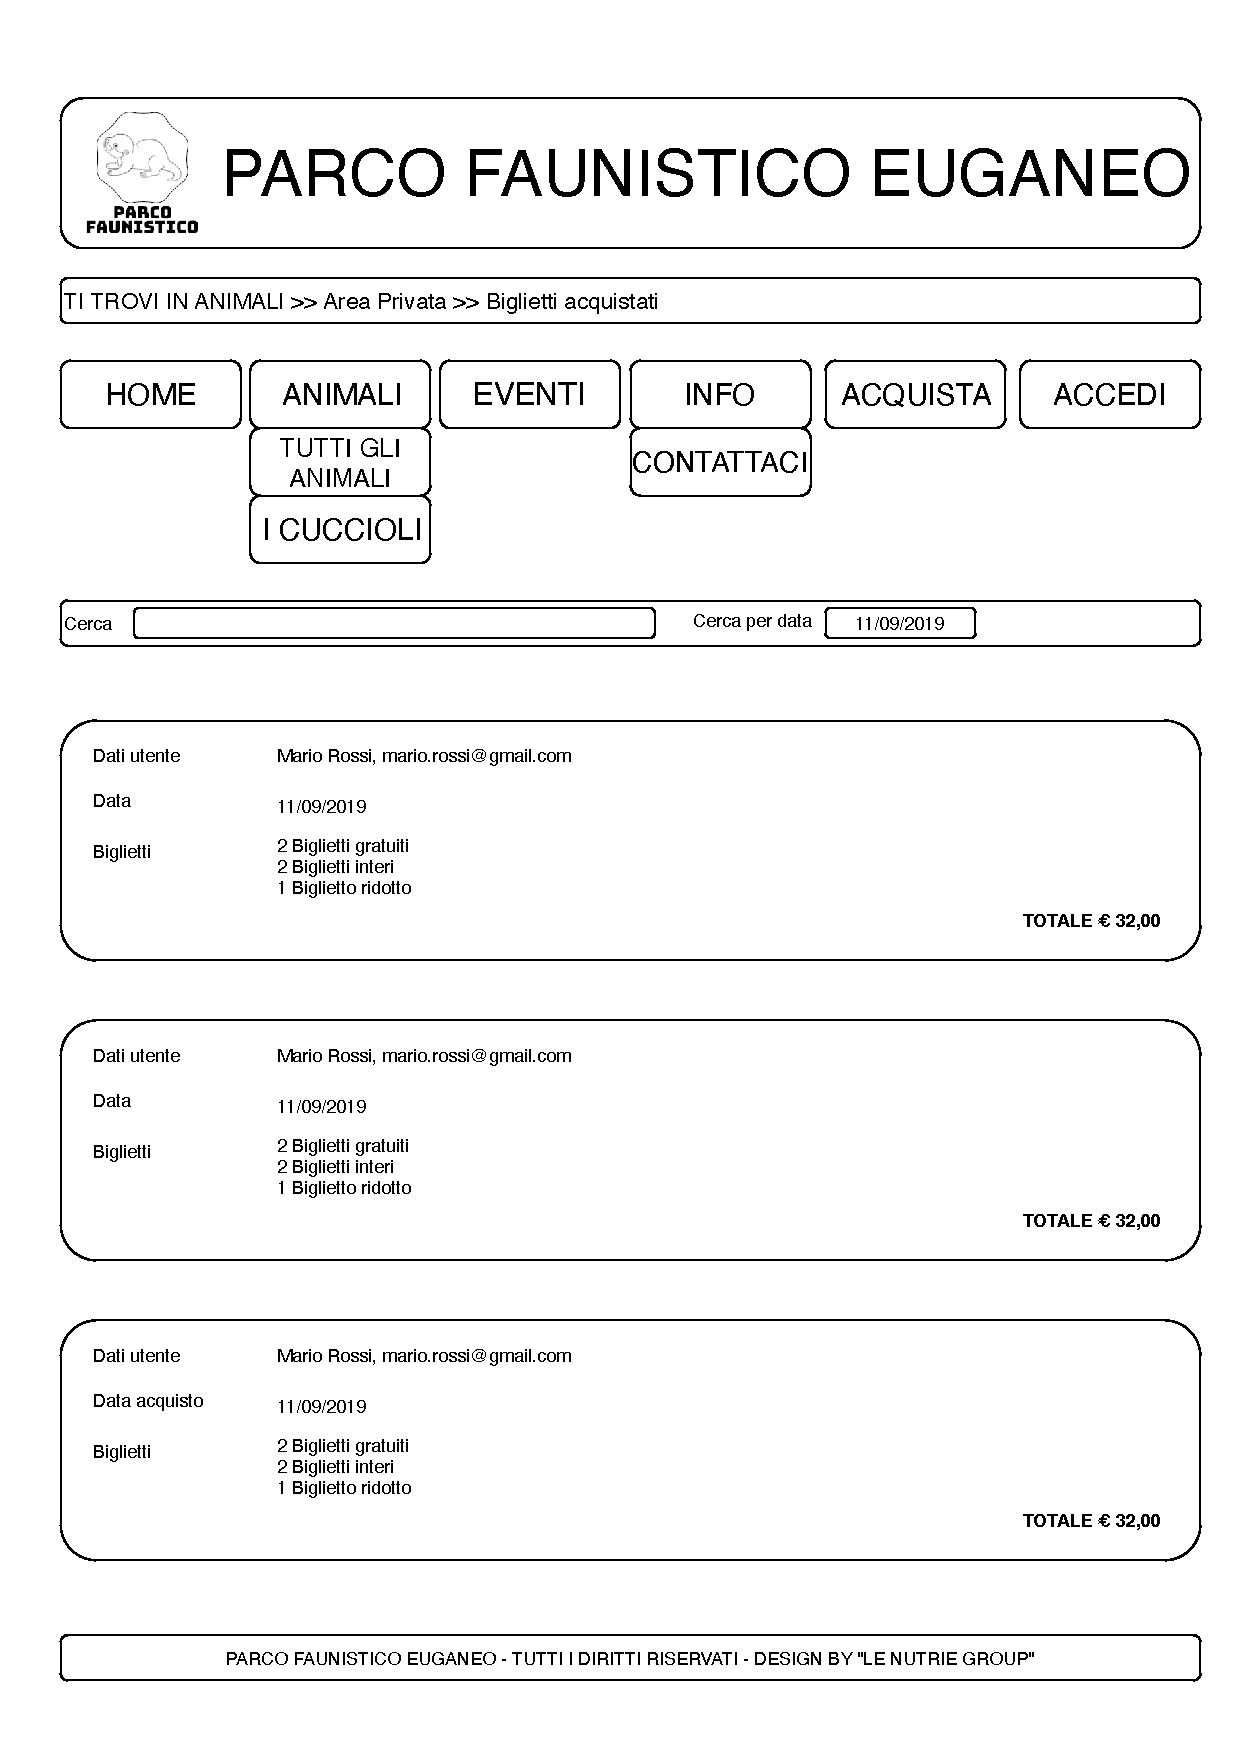
\includegraphics[width=\linewidth]{./../docs/Analisi/bozze/riepilogoAcquisti.pdf}
            \captionof{figure}{Area Privata - Riepilogo acquisti}
        \end{minipage}
        \hfill
        \begin{minipage}{0.5\linewidth}
            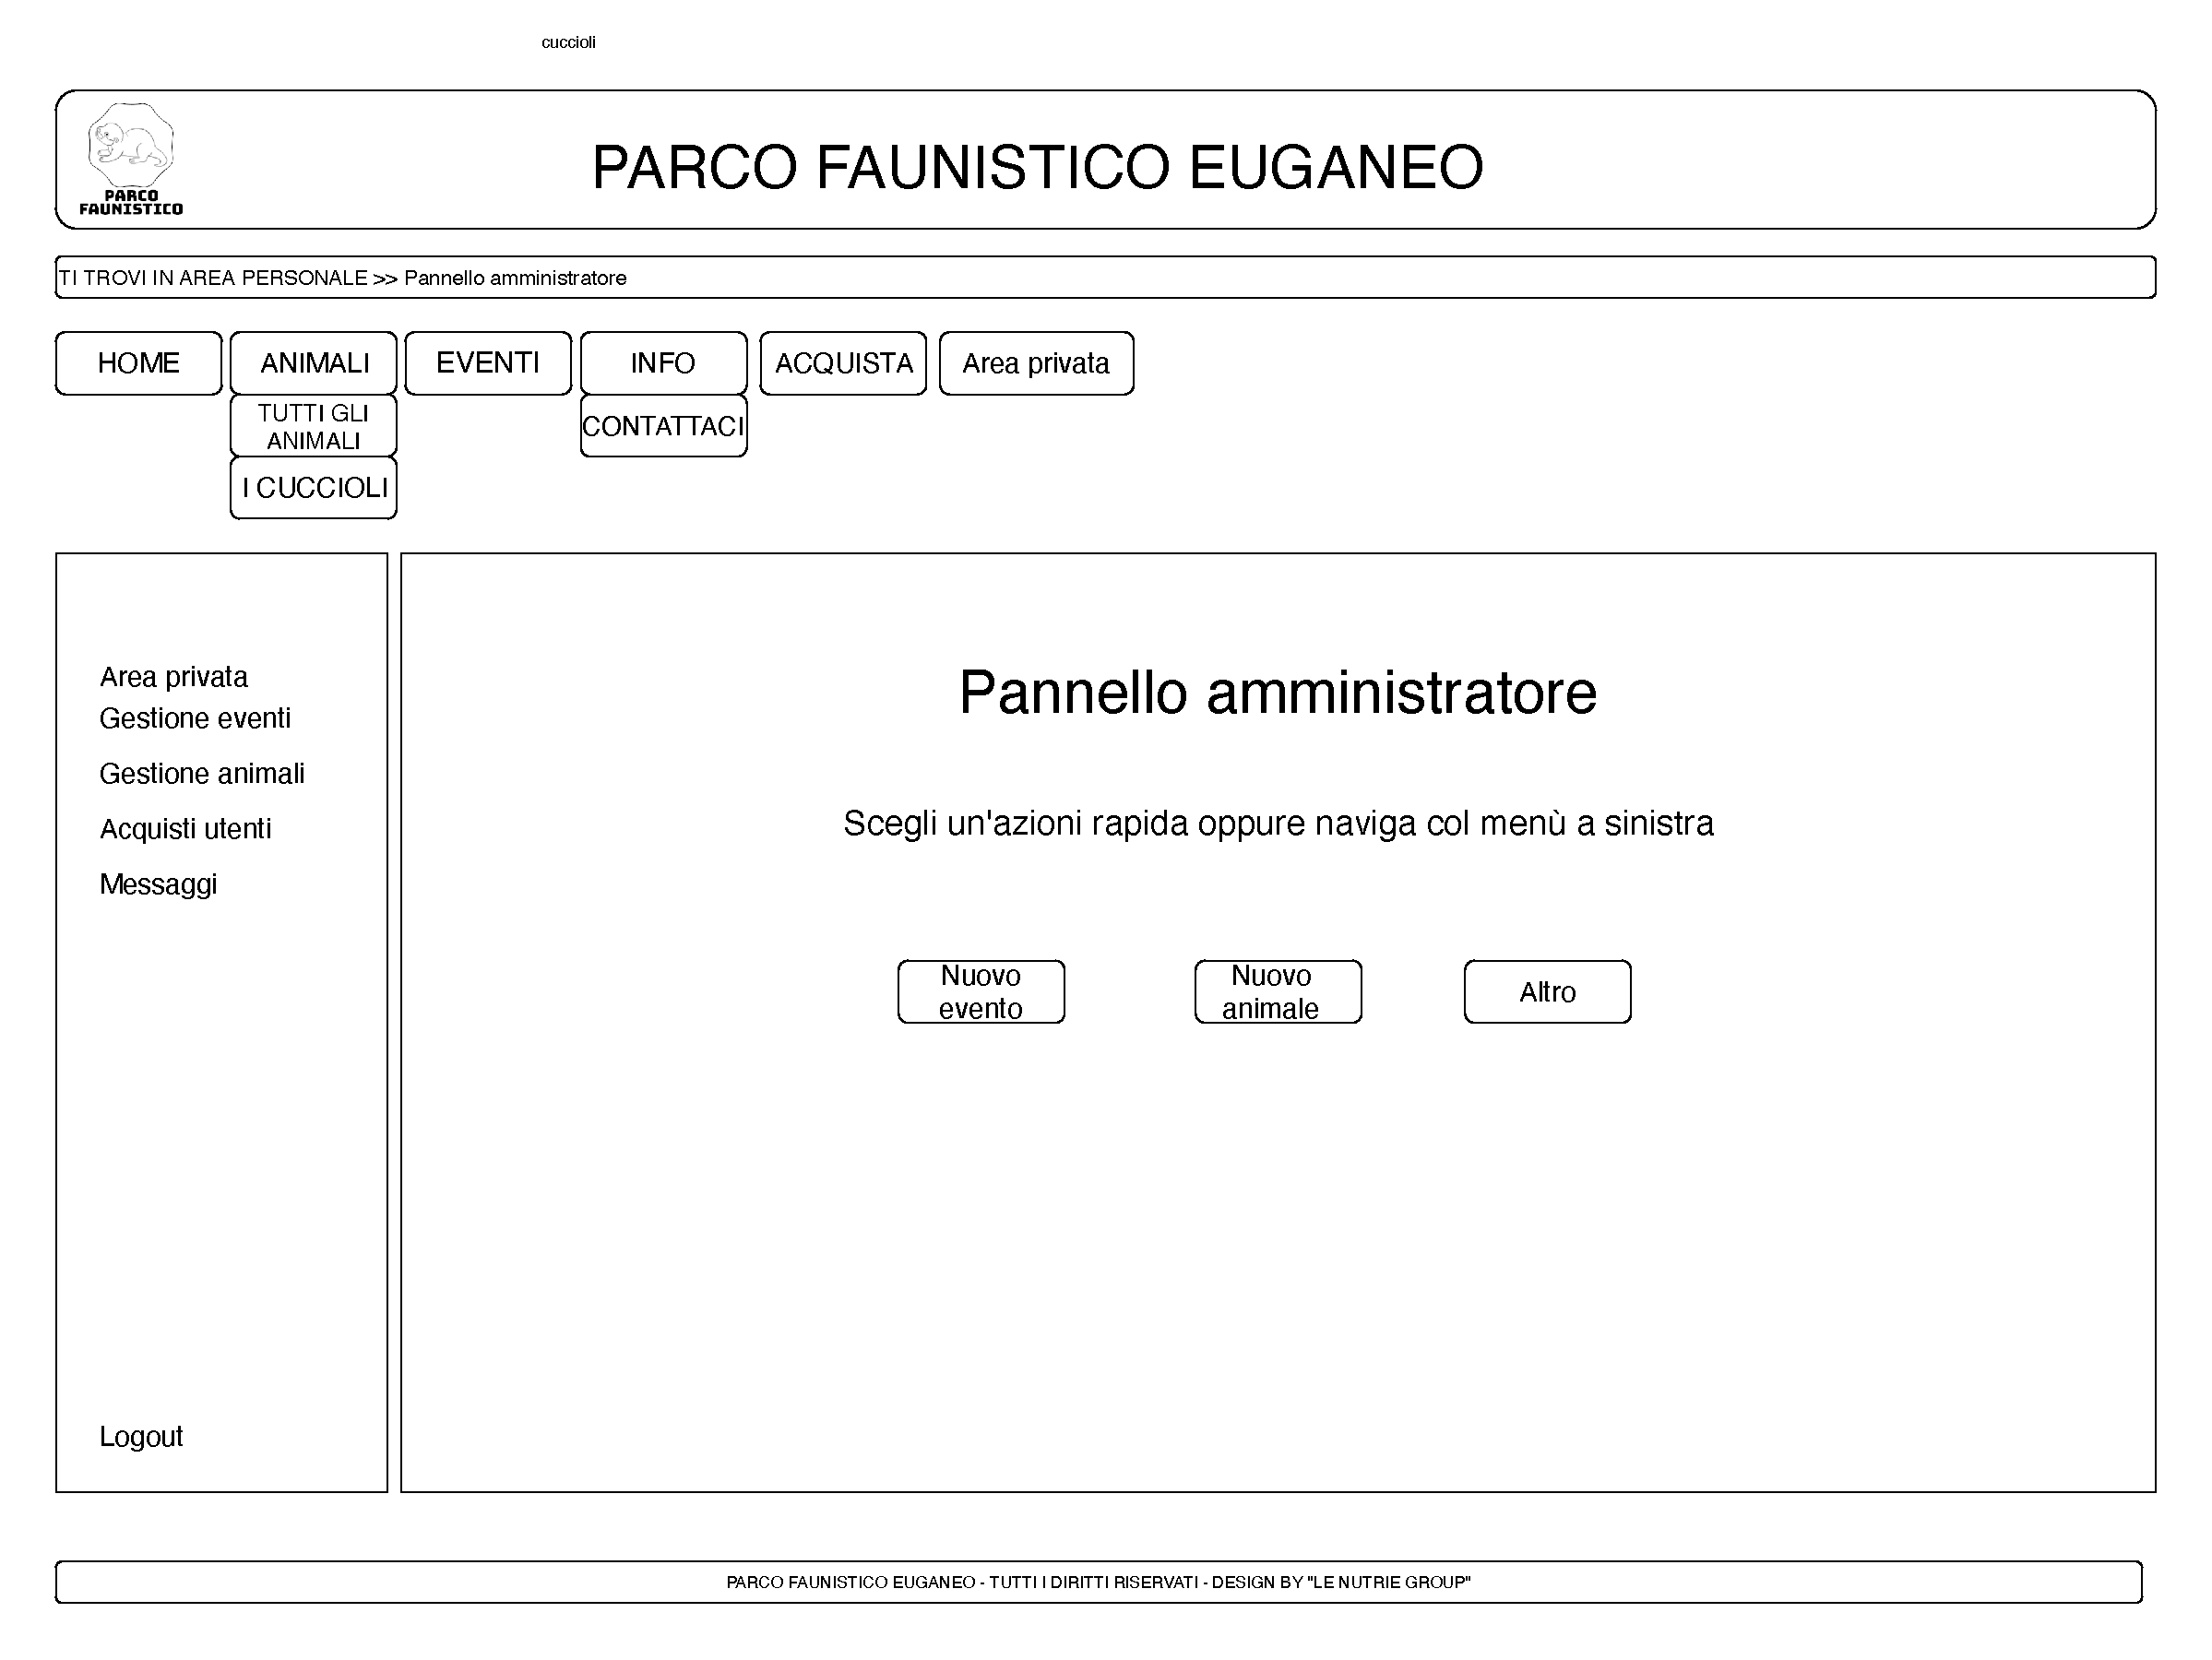
\includegraphics[width=\linewidth]{./../docs/Analisi/bozze/areaPrivata.pdf}
            \captionof{figure}{Area amministratore}
        \end{minipage}
    \end{center}
        
    La struttura della gerarchia del sito è suddivisa in pagine, alcune delle quali hanno delle sottopagine:
    \begin{itemize}
        \item Home;
        \item Animali:
            \begin{itemize}
                \item Tutti gli animali;
                \item Cuccioli
            \end{itemize}
        \item Eventi;
        \item Informazioni:
            \begin{itemize}
                \item Contatti (ancora al form per contattare l'amministratore)
            \end{itemize}
        \item Acquista;
        \item Pagina di Login;
        \item Pagina di Registrazione;
        \item Area privata (utente generico):
            \begin{itemize}
                \item Area personale;
                \item Biglietti Acquistati;
                \item Eventi Prenotati;
                \item Messaggi Personali;
                \item Dati Personali.
            \end{itemize}
            \item Area privata (utente amministratore):
                \begin{itemize}
                    \item Area amministratore;
                    \item Eventi;
                    \item Animali;
                    \item Acquisti;
                    \item Messaggi.
                \end{itemize}
            \item Pagina di inserimento nuovo animale (solo amministratore);
            \item Pagina di inserimento nuovo evento (solo amministratore).
    \end{itemize}
    \subsection{Database}

    \begin{figure}[H]
        \centering
        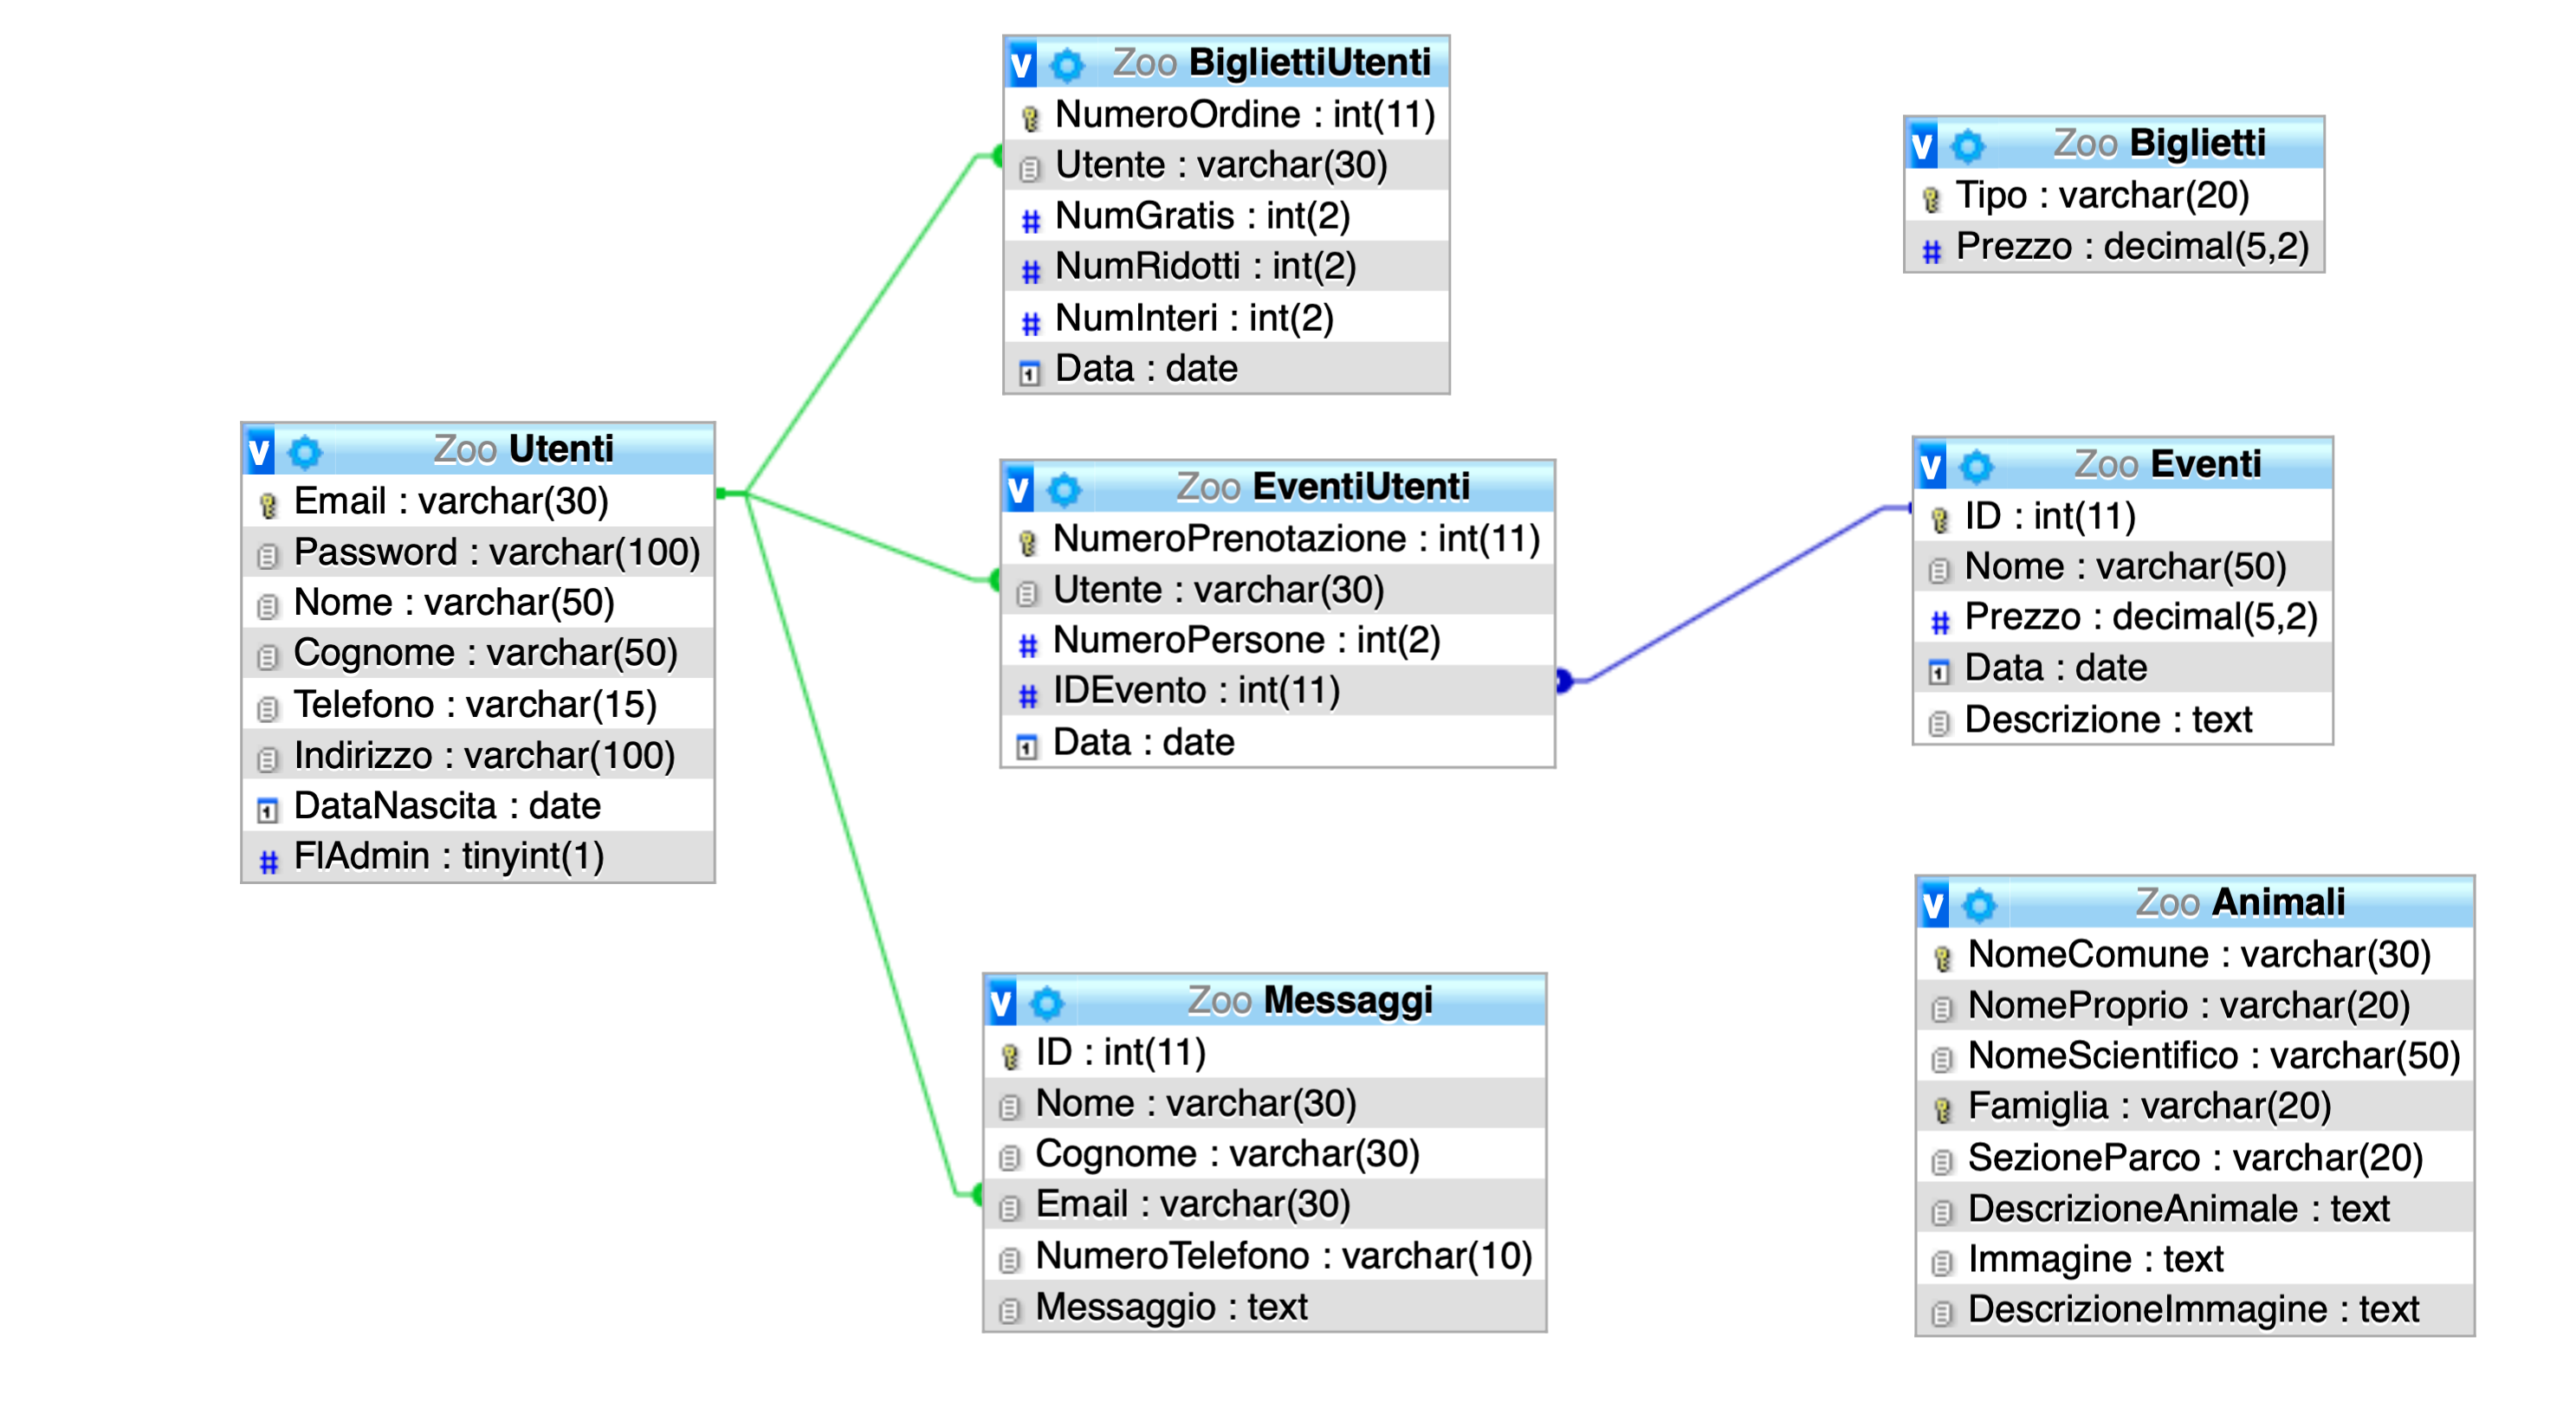
\includegraphics[width=15cm]{./img/database.png}
        \caption{Schema del database}  \label{fig:xray}
    \end{figure}
\pagebreak